\documentclass[border=4pt,12pt]{standalone}
% House style for redrawn exam diagrams (diagram-v4: 0.4pt lines, filled -latex arrows, fine dashes; stipple and hatching drawn as real dots/lines (no PDF/SVG patterns, so they render in every browser and at any scale); transparent background). Every figure \input's this.
\usepackage{amsmath,amssymb}
\usepackage{txfonts}
\usepackage{pdfrender,xcolor}
% \halo{text}: label on shading. The shading stops just around each letter's outline (a thin knock-out that follows the
% glyphs, like the papers' typesetting), never a box. Owner: "I don't want a box around the text".
\newcommand{\halo}[1]{\leavevmode\rlap{\pdfrender{TextRenderingMode=2,LineWidth=2.2pt,LineJoinStyle=1,StrokeColor=white,FillColor=white}#1}#1}
\usepackage{tikz,pgfplots}
\pgfplotsset{compat=1.18}
\usetikzlibrary{arrows.meta,calc,angles,quotes,patterns,patterns.meta,intersections,positioning,decorations.markings,shapes.geometric}
% Stipple and hatching are drawn as actual dots / lines clipped to the region (path picture), NOT as pattern fills:
% SVG <pattern> fills vanish or blur when browsers scale the image, so the owner could not see the shading.
% Each dot is a 0.72pt square (keeps SVGs small; reads as a dot at print size). Dots sit on one global staggered grid, so neighbouring regions line up.
\makeatletter
\newdimen\ex@x \newdimen\ex@y \newdimen\ex@xa \newdimen\ex@ya \newdimen\ex@xb \newdimen\ex@yb \newcount\ex@row
\def\exam@stipplecolor{black!75}\def\exam@dotr{0.42pt}\def\exam@dotgap{2.5}
\def\ex@rowdots{\ifdim\ex@x<\ex@xb \pgfpathrectangle{\pgfqpoint{\dimexpr\ex@x-0.36pt\relax}{\dimexpr\ex@y-0.36pt\relax}}{\pgfqpoint{0.72pt}{0.72pt}}\advance\ex@x by \exam@dotgap pt\relax\expandafter\ex@rowdots\fi}
\def\exam@stipple{%
  \pgftransformreset% dots are sized in real points even inside scaled pictures
  \pgfpointanchor{path picture bounding box}{south west}\ex@xa=\pgf@x \ex@ya=\pgf@y
  \pgfpointanchor{path picture bounding box}{north east}\ex@xb=\pgf@x \ex@yb=\pgf@y
  \pgfsetfillcolor{\exam@stipplecolor}\pgfmathsetmacro\ex@h{\exam@dotgap/2}%
  \pgfmathtruncatemacro\ex@r{floor(\ex@ya/\ex@h)-1}\ex@row=\ex@r\relax
  \ex@y=\ex@r\dimexpr\ex@h pt\relax
  \loop\ifdim\ex@y<\ex@yb
    \pgfmathtruncatemacro\ex@c{floor(\ex@xa/\exam@dotgap)-1}\ex@x=\ex@c\dimexpr\exam@dotgap pt\relax
    \ifodd\ex@row \advance\ex@x by \ex@h pt\fi
    \ex@rowdots
    \advance\ex@y by \ex@h pt \advance\ex@row by 1
    \ifnum\numexpr\ex@row-(\ex@row/4)*4\relax=0 \pgfusepath{fill}\fi% flush every 4 rows: bounded TeX memory, few clip copies in the SVG
  \repeat\pgfusepath{fill}}
\newdimen\ex@d
\def\exam@hatch#1{% #1 = 1 for /, -1 for \ ; lines 45 degrees, 3pt apart
  \pgftransformreset
  \pgfpointanchor{path picture bounding box}{south west}\ex@xa=\pgf@x \ex@ya=\pgf@y
  \pgfpointanchor{path picture bounding box}{north east}\ex@xb=\pgf@x \ex@yb=\pgf@y
  \ex@d=\dimexpr\ex@yb-\ex@ya\relax \ex@x=\dimexpr\ex@xa-\ex@d\relax
  \loop\ifdim\ex@x<\ex@xb
    \ifnum#1>0 \pgfpathmoveto{\pgfqpoint{\ex@x}{\ex@ya}}\pgfpathlineto{\pgfqpoint{\dimexpr\ex@x+\ex@d\relax}{\ex@yb}}%
    \else \pgfpathmoveto{\pgfqpoint{\ex@x}{\ex@yb}}\pgfpathlineto{\pgfqpoint{\dimexpr\ex@x+\ex@d\relax}{\ex@ya}}\fi
    \advance\ex@x by 4.24pt
  \repeat
  \pgfsetlinewidth{0.4pt}\pgfsetstrokecolor{black}\pgfusepath{stroke}}
\def\examstipple{\exam@stipple}\def\examhatch{\exam@hatch}\def\examsetstipplecolor#1{\def\exam@stipplecolor{#1}}\def\examsetdotgap#1{\def\exam@dotgap{#1}}
\makeatother
% (legacy pattern kept for old files)
% staggered stipple like the NESA papers' dotted shading
\pgfdeclarepatternformonly{exam stipple}{\pgfpointorigin}{\pgfqpoint{2.2pt}{2.2pt}}{\pgfqpoint{2.2pt}{2.2pt}}{%
  \pgfpathcircle{\pgfqpoint{0.55pt}{0.55pt}}{0.42pt}\pgfpathcircle{\pgfqpoint{1.65pt}{1.65pt}}{0.42pt}\pgfusepath{fill}}
\tikzset{
  every picture/.style={line width=0.6pt, >={Latex[length=2mm,width=1.3mm]}},
  curve/.style={line width=0.6pt},
  open arrow/.style={-{Latex[length=2mm,width=1.3mm]}},  % owner: filled -latex heads everywhere, no open chevrons
  aux/.style={dash pattern=on 2pt off 1.5pt, line width=0.6pt},
  shade/.code={\def\exA{#1}\def\exB{none}\ifx\exA\exB\else\pgfkeysalso{fill=black!18}\fi},
  shade/.default=on,
  shade dots/.style={fill=none, path picture={\examstipple}},
  stipple color/.code={\examsetstipplecolor{#1}},
  stipple gap/.code={\examsetdotgap{#1}},
  shade dense dots/.style={fill=none, stipple gap=1.6, path picture={\examstipple}},
  shade hatch/.style={fill=none, path picture={\examhatch{1}}},
  shade hatch reverse/.style={fill=none, path picture={\examhatch{-1}}},
  shade solid/.style={fill=black},
  pt/.style={circle, fill, inner sep=1.1pt},
  open pt/.style={circle, draw, fill=white, inner sep=1.1pt},
}
\pgfplotsset{
  exam axes/.style={axis lines=middle, axis line style={->}, xlabel={$x$}, ylabel={$y$},
    xlabel style={anchor=west}, ylabel style={anchor=south}, tick label style={font=\small},
    every axis plot/.append style={line width=0.6pt, black}, samples=200, clip=false,
    enlargelimits=false, axis on top},
}

\begin{document}
% 2024 Ascham AT4 Q36 solution: y=f'(x) sketched on the question's graph of f (crop pixel units, y down; question graph offset 28 px)
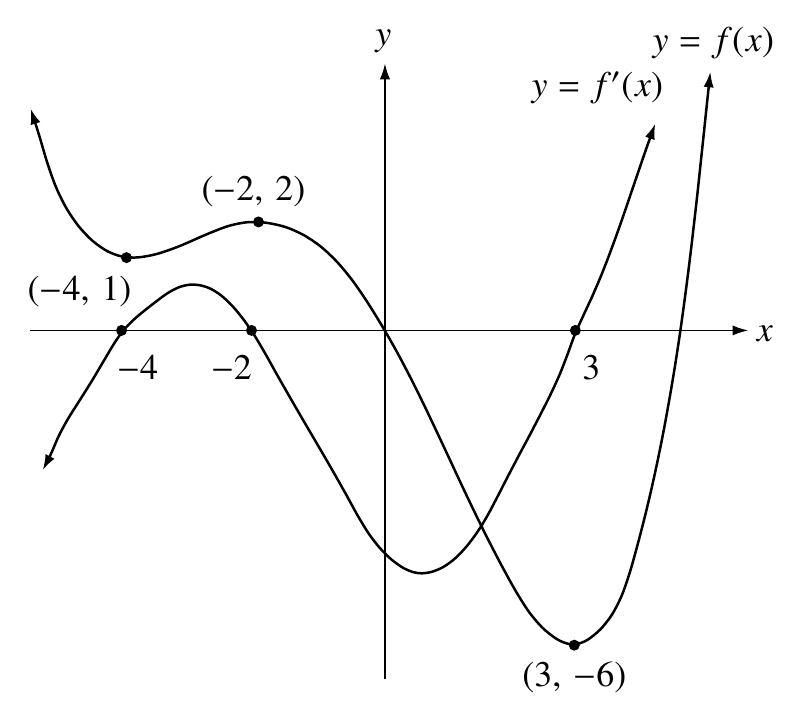
\begin{tikzpicture}[x=0.0127cm,y=-0.0127cm, every node/.style={inner sep=0pt, font=\fontsize{13}{15}\selectfont}]
  \draw[->] (44,317) -- (763,317);
  \draw[->] (399.5,666) -- (399.5,50);
  \node[anchor=west] at (769,320) {$x$};
  \node[anchor=south] at (398,40) {$y$};
  \draw[<->,line width=0.9pt] plot[smooth] coordinates {(45,95) (53.41,121.4) (61.74,149.4) (70.32,173.4) (80.72,194.6) (93.24,213) (107.2,227.6) (121.9,237.8) (136.2,243) (152.1,244) (171.4,240.5) (193.9,232.7) (220.1,221.3) (242.4,212.7) (261.5,208.8) (280,209.2) (299.7,213.5) (318.2,221.6) (335.5,233.3) (351.9,248.8) (367.7,268) (382.7,290) (397.6,314.2) (411.9,339.3) (425.3,364.8) (438.4,391.2) (451.2,418.1) (464,445.4) (476.9,473.1) (489.8,500.1) (502.7,526.2) (516.2,552.2) (530.3,577.7) (543.5,598.5) (557.2,614.6) (571.4,625.8) (582.7,630.5) (591.8,630.7) (602.2,626.5) (614.8,616.3) (626.5,601.5) (636.3,582.4) (644.5,558.9) (652.3,531.1) (659.6,502.9) (666.4,474.3) (672.7,445.3) (678.5,416.3) (683.8,387.2) (688.8,357.8) (693.4,328.3) (697.6,298.8) (701.6,268.8) (705.3,239.2) (708.8,209.2) (712.2,179.2) (715.4,149) (718.6,118.9) (721.8,88.29) (725,58)};
  \foreach \p in {(273,208.5),(140.9,244.2),(588.9,631.9)} \fill \p circle (5.5);
  \node at (268,178) {$(-2,\,2)$};
  \node at (94,278) {$(-4,\,1)$};
  \node at (589,664) {$(3,\,-6)$};
  \node at (728,30) {$y=f(x)$};
  \draw[<->,line width=0.9pt] plot[smooth] coordinates {(57,457) (64.83,441.7) (73.28,422.4) (82.4,405.5) (94.12,386.9) (106,368) (117.7,348.3) (129.1,329.3) (138.7,315.9) (150.5,304.2) (166.5,291.2) (182.1,279.7) (193.7,273.7) (204.1,271.3) (214.3,271.8) (224.6,275.1) (235.5,281.9) (247,292.7) (258.6,306.9) (269.8,323.4) (280.6,341.7) (291.8,361.8) (303.4,382.1) (315,402.2) (327,422.7) (338.7,442.7) (350.4,463) (361.7,483.1) (372.6,502.9) (383.1,520) (393.8,534) (405.4,545.7) (417.3,554.3) (427.7,558.8) (436.6,560) (447.1,558.3) (458.2,553.5) (469.4,545.3) (480.8,533.5) (491.9,518.8) (502.2,502) (512.3,482.9) (522.8,462.4) (533.6,441.8) (544.7,421) (555.3,400.6) (565.5,380.3) (574.4,360.8) (581.9,341.6) (589.4,321.2) (597.7,302.7) (607.1,282.4) (615.8,262.1) (624,241.1) (631.8,219.8) (639.4,198.1) (647,175.8) (654.6,153.5) (662.2,131.5) (670,110)};
  \foreach \p in {(136,317),(266,317),(590,317)} \fill \p circle (5.5);
  \node at (152,354) {$-4$};
  \node at (246,354) {$-2$};
  \node at (606,354) {$3$};
  \node at (612,74) {$y=f'(x)$};
\end{tikzpicture}
\end{document}
